%% \chapter[htoc-titlei][hhead-titlei]{htitlei}
%% -----------------------------------------------------------------------------
\chapter[Theoretical Framework][Theoretical Framework]{Theoretical Framework} \label{ch:theory}

This chapter outlines the theoretical groundwork for the rest of the thesis.
An overview of the Standard Model of particle physics (SM) is given in Section~\ref{sec:theory_sm}, followed by the electroweak symmetry breaking mechanism involving the Higgs boson in Section~\ref{sec:theory_higgs}.
Finally, Section~\ref{sec:theory_vbs} will go into detail on the interests of electroweak vector boson scattering (VBS).

\section{Introduction to the Standard Model} \label{sec:theory_sm}
The Standard Model of particle physics serves as a mathematical description of the fundamental particles of the universe and their interactions.
It has been developed over the course of the past century, incorporating both predictions from theory and results from experiments.
All in all, the SM has proven to be very accurate in describing the particle interactions seen in experiments, as can be seen in the summary plot in Figure~\ref{fig:theory_sm_meas} comparing ATLAS measurements to their SM predictions.
%Nearly all measurements are consistent with the SM predictions

\begin{figure}
  \centering
  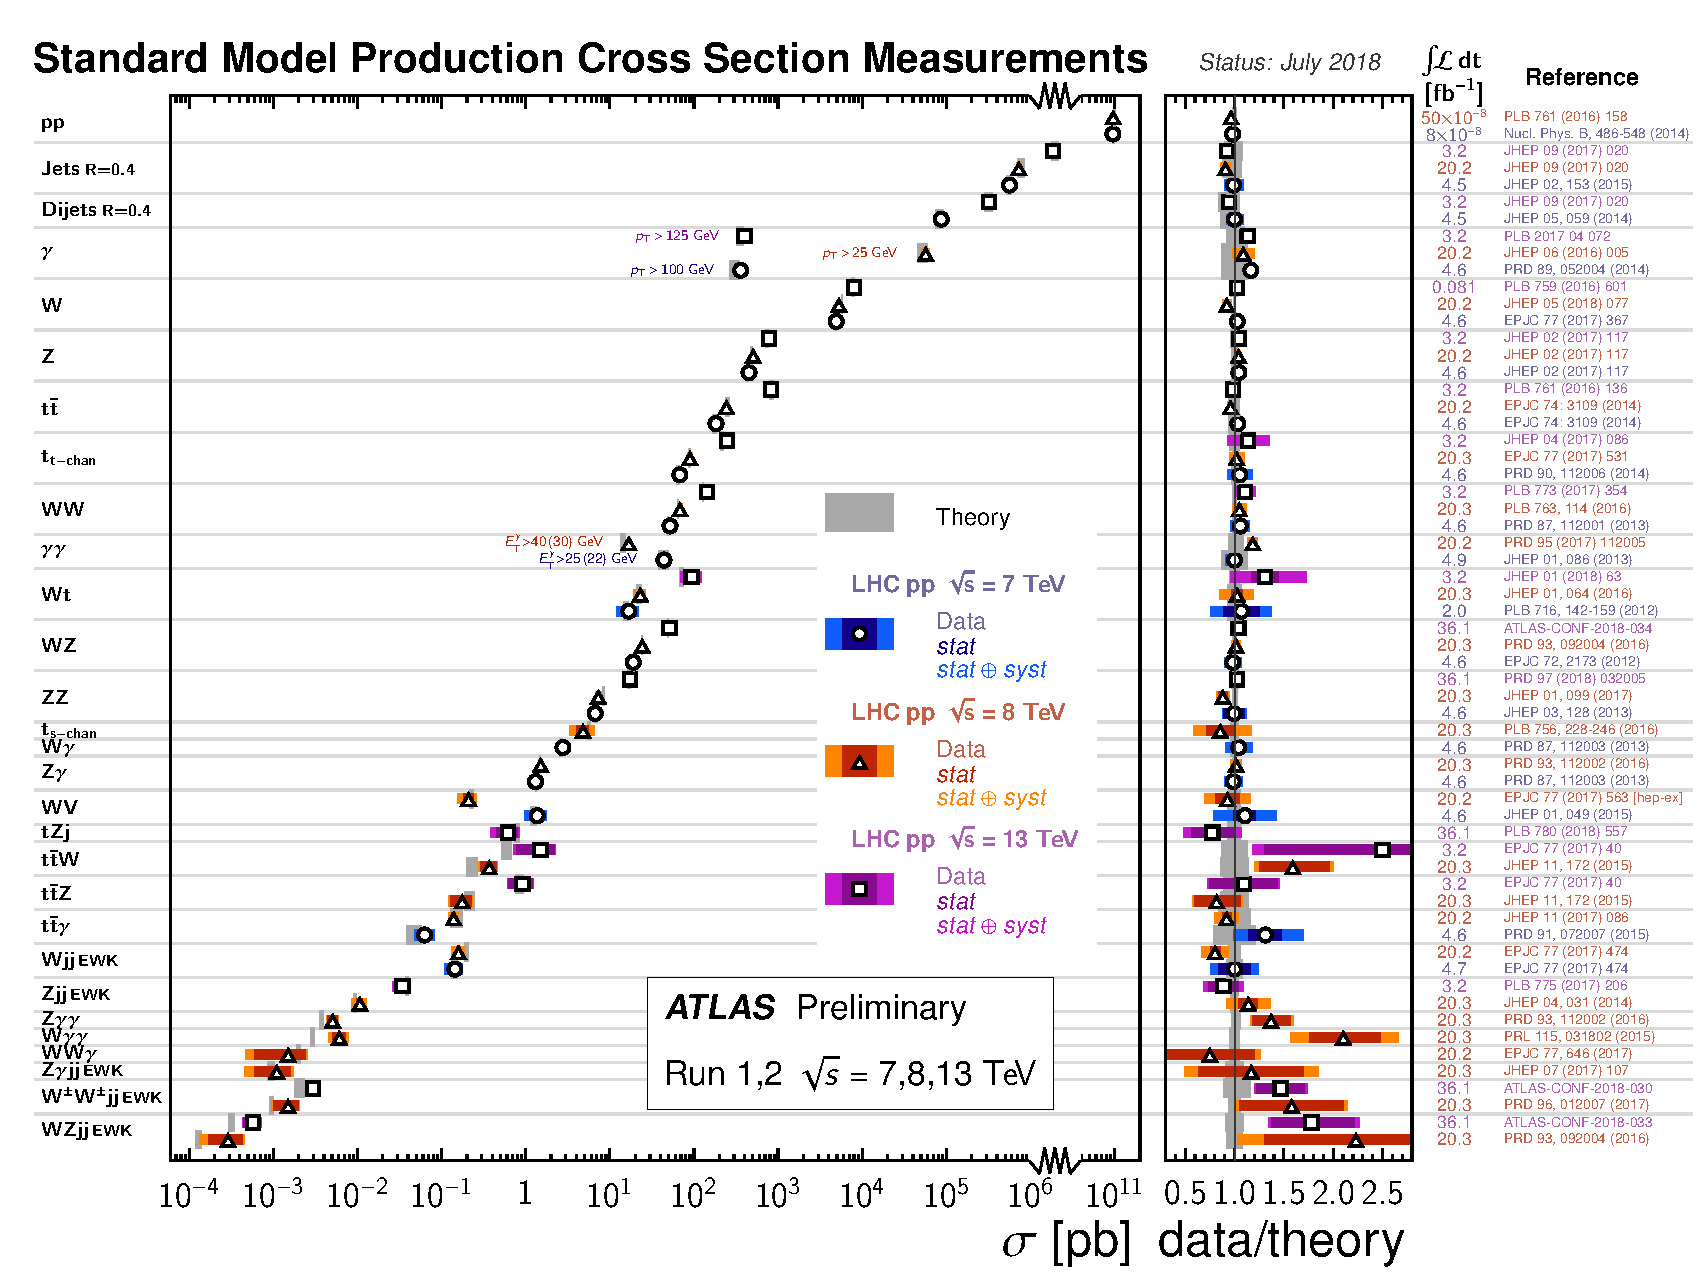
\includegraphics[width=\textwidth]{figs/theory/ATLAS_sm_measurements}
  \caption[Summary of several Standard Model total and fiducial production cross section measurements compared to the corresponding theoretical predictuions calculated at NLO or higher. The dark colored error bar represents the statistical uncertainty, and the light colored error bar represents the full uncertainty (including systematic and luminosity uncertainties). The data/theory ratio, luminosity used and reference for each measurement are also shown.]{Summary of several Standard Model total and fiducial production cross section measurements compared to the corresponding theoretical predictuions calculated at NLO or higher. The dark colored error bar represents the statistical uncertainty, and the light colored error bar represents the full uncertainty (including systematic and luminosity uncertainties). The data/theory ratio, luminosity used and reference for each measurement are also shown~\cite{2019.atlas-summary-plots}.}
  \label{fig:theory_sm_meas}
\end{figure}

The SM is a quantum field theory (QFT)~\cite{1995.Weinberg, 1995.Peskin} in which the fundamental particles are represented as excited states of their corresponding fields.
The spin-$\frac{1}{2}$ fermionic fields give rise to the quarks and leptons comprising ordinary matter, the spin-1 fields correspond to the electroweak bosons and the gluon which mediate the electroweak and strong forces, respectively, and finally the scalar Higgs field is responsible for electroweak symmetry breaking.
The excitations and interactions of the fields are governed by the SM Lagrangian, which is invariant under local transformations of the group $\gtsu{3}\times\gtsu{2}\times\gtu{1}$.
%\TODO{need more detail/refinement here}

The first quantum field theory to be developed was quantum electrodynamics (QED)~\cite{1950.Feynman.QED}, which describes the electromagnetic interaction.
The theory predicts the existence of a $\gtu{1}$ gauge field that interacts with the electrically charged fermions.
This field corresponds to the photon.
A key aspect of QED is that it is perturbative: the coupling constant $\alpha = e^2/4\pi$ is small, where $e$ is electrical charge of the field, allowing for the use of perturbation theory in calculations.
In this case, calculations can be written as a power series in $\alpha$, where successive higher order terms contribute less to the final result.
The accuracy of perturbative calculations is an essential tool for being able to make predictions from the SM.
%\TODO{renormalizability here?}

The strong interaction---the theory of quarks and gluons---has also been described using QFT as quantum chromodynamics (QCD).
%QCD is the theory of quarks and the associated strong force-carrier the gluon.
The symmetry group for QCD is $\gtsu{3}$, and its eight generators correspond to the eight differently charged, massless gluons~\cite{1965.Han-Nambu.Propose-color}.
Unlike in QED, which has the familiar positive and negative electric charges, the strong force has three ``colors''.
Color charge combined with the non-Abelian nature of $\gtsu{3}$, which allows the gluons to interact with each other, result in the most well-known property of QCD: color confinement.
In order to increase the separation between two color-charged quarks, the amount of energy required increases until it becomes energetically favorable to pair-produce a new quark-antiquark pair, which then bind to the original quarks.
The end result of this is that only color-neutral objects exist in isolation. % and it is responsible for the hadronic jets in experiments.
What this means for the strong coupling constant $\alpha_s$ is that its value at the low energies where confinement occurs is large, on the order of $\alpha_s\sim 1$.
The consequense of this is that perturbation theory cannot be used to approximate these interactions.
While this appears at first to be a critical problem for prediction, fortunately it turns out that $\alpha_s$ ``runs'', or decreases in magnitude at higher energy~\cite{1973.asymptotically-free-i, 1974.asymptotically-free-ii}.
This so-called ``asymptotic freedom'' allows QCD to be calcualted perturbatively~\cite{1973.strong-perturbation} at energies accessible by collider experiments including the LHC.
%A second important property of the QCD is that, unlike in QED, the coupling constant $\alpha_s$ is large at low energies where confinement occurs, and thus it cannot be described accurately using perturbation theory.
%Fortunately, $\alpha_s$ ``runs'', or decreases at higher energy scales~\cite{1973.asymptotically-free-i, 1974.asymptotically-free-ii}; this allows QCD to be calculated perturbatively~\cite{1973.strong-perturbation} at energies accessible by collider experiments including the LHC.

The last gauge field corresponds to the weak interaction.
Ultimately, the weak $\gtsu{2}$ and the electromagnetic $\gtu{1}$ mix to form the $\gtsu{2}\times\gtu{1}$ \emph{electroweak} (EWK) interaction~\cite{1959.Salam.electroweak, 1959.Glashow.vector-mesons}.
A more detailed description of the mixing will be discussed in conjunction with electroweak symmetry breaking (EWSB) in Section~\ref{sec:theory_higgs}; however, a summary of the resulting EWK interaction is presented here, at the risk of some repeated information to follow.
There are three weak isospin bosons arising from the $\gtsu{2}$ group ($W_{\mu}^1$, $W_{\mu}^2$, and $W_{\mu}^3$) and one weak hypercharge boson from the $\gtu{1}$ group ($B_{\mu}$).
The $W_3$ and $B$ bosons mix according to the weak mixing angle $\theta_W$ to form the $Z$ boson and the photon according to
\begin{equation}
  \begin{pmatrix}
  \gamma\\
  Z
  \end{pmatrix}
  = 
  \begin{pmatrix}
  \cos{\theta_W} & \sin{\theta_W} \\
  -\sin{\theta_W} & \cos{\theta_W}
  \end{pmatrix}
  \begin{pmatrix}
  B_{\mu} \\
  W_{\mu}^3
  \end{pmatrix}\,.
  \label{eq:weak_mixing}
\end{equation}
The value of $\theta_W$ is not predicted by the SM; it is one example of an experimental input to the theory, measured to be $\sin^2{\theta_W} = 0.23153\pm0.00016$~\cite{2006.weak-mixing}.
The charged $W^{\pm}$ bosons are a mixture of the remaining $W_{\mu}^1$ and $W_{\mu}^2$ bosons:
\begin{equation}
  W^{\pm} = \frac{1}{\sqrt{2}}(W_{\mu}^1 \mp iW_{\mu}^2)\,.
  \label{eq:w_mixing}
\end{equation}
Unlike the photon (and the gluon of QCD), the $W^\pm$ and $Z$ bosons are massive.
This means that even though $\gtsu{2}$ is non-Abelian, the range of interaction is short and confinement does not occur.
Lastly, the EWK interaction is chiral, only coupling to the left-handed component of the fermion fields.

One final field remains within the SM: the scalar Higgs field.
It was originally proposed in the 1960's to explain the masses of the $W^{\pm}$ and $Z$ bosons~\cite{1964.Englert.symmetry_breaking, 1964.Higgs.Broken_Symmetries_1, 1964.Higgs.Broken_Symmetries_2} and is the mechanism for the EWSB process.
The particle associated with the field is a massive scalar boson, the Higgs boson, which was recently discovered by ATLAS and CMS in 2012~\cite{HIGG-2012-27, CMS-HIG-12-028} with a mass of $125\gev$.


%\subsection{Electroweak mixing}\label{theory:ewk_mixing}
%\begin{itemize}
%  \item intro: theory+experimental motivation, four forces, blah
%  \item paragraph about what QFT is
%  \item Gauge invariance, renormalizibility of lagrangian (useful for the WW stuff later)
%  \item Electromagnetism - QED, $\alpha$, perturbation theory
%  \item Electroweak - mixing with EM, W/Z/$\gamma$, self-interacting is important for T/QGC, left handed
%  \item Strong - confinement, asymptotic freedom
%  \item Higgs - introduce it here w/ separate section after, source of mass for fermion/boson, discovery reference
%\end{itemize}


\section{Electroweak symmetry breaking and the Higgs boson} \label{sec:theory_higgs}
When the theory of the electroweak interaction was first developed \cite{1959.Glashow.vector-mesons, 1959.Salam.electroweak},
the $W$ and $Z$ bosons were predicted to be massless (a typical mass term in the Lagrangian would violate the SU(2) symmetry).
However, these were experimentally observed to have masses...


%\section{Diboson physics}\label{sec:theory_diboson}
%two bosons


\section{Electroweak vector boson scattering}\label{sec:theory_vbs}
Due to the non-Abelian nature of the EWK interaction, the associated gauge bosons are allowed to self-interact.
This results in triple and quartic couplings of gauge bosons (TGCs and QGCs, respectively).
The SM allowed TGCs are the $WW\gamma$ and $WWZ$ vertices, which can be measured experimentally via diboson production or through vector boson fusion (VBF).
QGCs predicted by the model include $WWZ\gamma$, $WW\gamma\gamma$, $WWZZ$, and $WWWW$ vertices accessible in triboson production or via vector boson scattering (VBS)\footnote{Vector boson fusion and scattering typically refer to the $s$-channel and $t$-channel exchanges of a vector boson, respectively.  Since both deal with a similar $VV\rightarrow VV$ process, for the remainder of this thesis, \emph{vector boson scattering} will refer to both VBF and VBS.}~\cite{2017.multiboson-at-lhc}.
VBS processes are defined by a $VV\rightarrow VV$ signature, where $V$ represents one of the EWK gauge bosons ($W^{\pm}$, $Z$, or $\gamma$), as shown in Figure~\ref{fig:theory_generic_vbs}.
The actual interaction between the incoming and outgoing vector bosons can be mediated by the exchange of a virtual $V$, directly via a QGC (as in Figure~\ref{fig:theory_vbs_ewk}), or by the exchange of a Higgs boson (as in Figure~\ref{fig:theory_vbs_higgs}).

\begin{figure}[htbp]
  \centering
  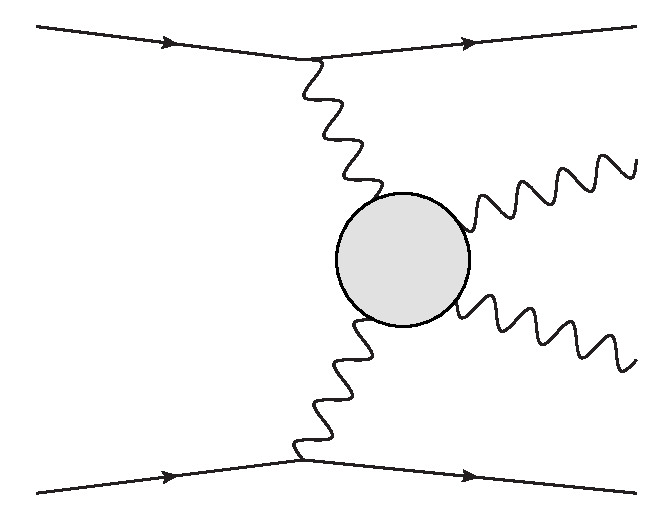
\includegraphics[width=.4\textwidth]{figs/theory/generic_vbs}
  \caption{Feynman diagram of a generic VBS process.  The gray circle represents any interaction with two incoming and two outgoing vector bosons, including any of the diagrams shown in Figures~\ref{fig:theory_vbs_ewk} and \ref{fig:theory_vbs_higgs}.}
  \label{fig:theory_generic_vbs}
\end{figure}

\begin{figure}[htbp]
  \centering
  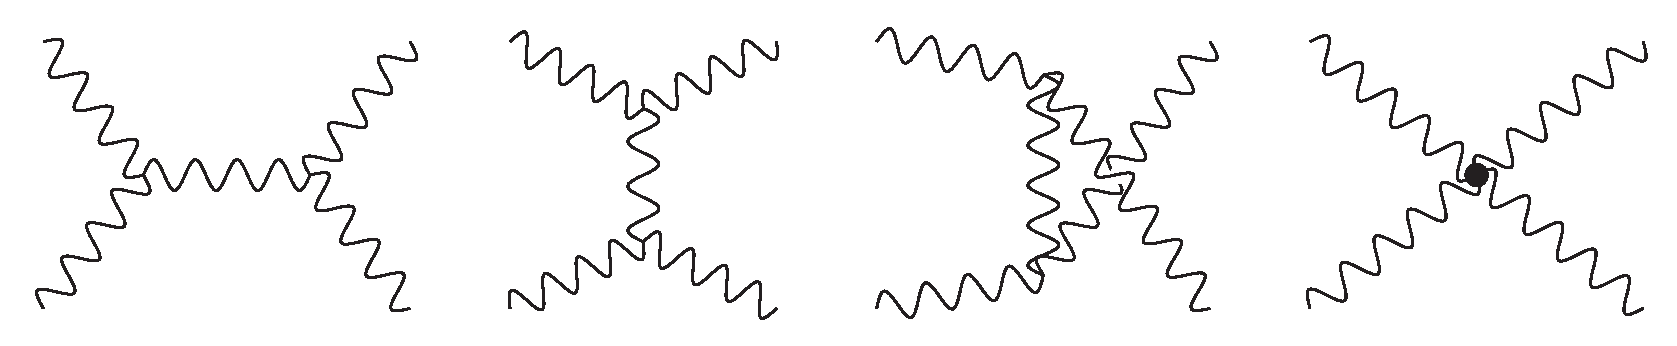
\includegraphics[height=.125\textheight]{figs/theory/vbs_ewk}
  \caption{Leading order $VV\rightarrow VV$ Feynman diagrams involving EWK bosons. From left to right: $s$-channel, $t$-channel, $u$-channel, and the quartic gauge coupling.}
  \label{fig:theory_vbs_ewk}
\end{figure}
\begin{figure}[htbp]
  \centering
  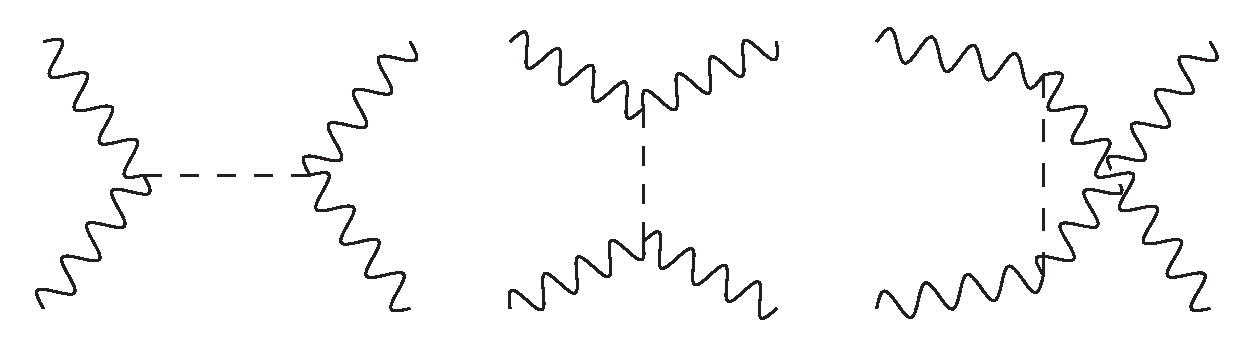
\includegraphics[height=.125\textheight]{figs/theory/vbs_higgs}
  \caption{Leading order $VV\rightarrow VV$ Feynman diagrams involving the exchange of a Higgs boson. From left to right: $s$-channel, $t$-channel, and $u$-channel.}
  \label{fig:theory_vbs_higgs}
\end{figure}

As detailed in the previous section, the Higgs mechanism produces three Goldstone bosons and a Higgs boson.
The Goldstone bosons are then ``eaten'' by the physical gauge bosons, giving them mass and consequently a longitudinal polarization\footnote{A massless spin-1 boson can have one of two transverse polarization states, while a massive spin-1 boson can also be longitudinally polarized.  As a result, only the massive $W^{\pm}$ and $Z$ bosons, and not the massless photon, are sensitive to EWSB.}.
In fact, according to the Electroweak Equivalence Theorem, the high-energy interactions of longitudinal gauge bosons can be accurately described by the Goldstone bosons of the EWSB mechanism~\cite{1997.ewk-equivalence}.
Thus, the scattering of the massive gauge bosons are inextricably linked to EWSB.

It turns out that without a light SM Higgs boson, the scattering amplitude of longitudinally polarized vector bosons grows with center-of-mass energy and ultimately violates unitarity above $\sqrt{s}\approx 1.2\tev$~\cite{1977.ben-lee-weak-interactions, 2009.strong-gauge-boson-scattering}.
Writing down the equations for the transverse and longitudinal polarization vectors for a gauge boson of mass $M_V$~\cite{1990.strong-ww-scattering}:
\begin{equation}
  \epsilon^{\mu}_{\pm} = \frac{1}{\sqrt{2}}(0,0,\pm i, 0)
\end{equation}
\begin{equation}
  \begin{aligned}
    \epsilon^{\mu}_L &= \frac{1}{M_V}(|\vec{p}|, 0, 0, E)\\
                    &= \frac{p^{\mu}}{M_V}+v^{\mu}
  \end{aligned}
  \label{eq:longitudinal_polarization}
\end{equation}
where $v^{\mu}$ is of the order $M_V/E$ and becomes small in the high energy limit, it can be seen that $\epsilon^{\mu}_{L}$ grows with the momentum of the boson $p^{\mu}$.
Therefore, the dominant contribution to the VBS process at high energy comes from the longitudinally polarized gauge bosons~\cite{2012.vbs-thesis-oord}.

% reference diagrams above, then do the matrix element thing (StrongGaugeBosonScatteringTheory.pdf sec 1.1), and cite the figure below
The high-energy behavior of longitudinally polarized vector boson scattering can be explored in the case of opposite-sign $W^{+}W^{-}\rightarrow W^{+}W^{-}$ scattering.
In the high-energy limit ($s \gg M_W^2, M_H^2$), the amplitude of $W^{+}W^{-}$ scattering without considering the Higgs contributions (the relevant diagrams in Figure~\ref{fig:theory_vbs_ewk}) can be written as~\cite{2009.strong-gauge-boson-scattering}:
\begin{equation}
  \mathcal{M}_{\textrm{gauge}} = -\frac{g^2}{4M_W^2}u+\mathcal{O}\Bigg(\bigg[\frac{E}{M_W}\bigg]^0\Bigg)
  \label{eq:theory_longitudinal_m_gauge}
\end{equation}
where $g$ is the EWK coupling and $u$ is one of the Mandelstam variables (the others being $s$ and $t$).
The $\mathcal{O}(E^4)$ terms cancel out between the TGC and QGC diagrams~\cite{2012.vbs-thesis-oord}.
What is left is an amplitude proportional to $E^2$ that diverges as $E/M_W\rightarrow\infty$.
However, the amplitude from the diagrams involving the Higgs boson (the relevant diagrams in Figure~\ref{fig:theory_vbs_higgs}) is:
\begin{equation}
  \mathcal{M}_{\textrm{Higgs}} = -\frac{g^2}{4M_W^2}\bigg[\frac{(s-M_W^2)^2}{s-m_H^2}+\frac{(t-M_W^2)^2}{t-M_H^2}\bigg]
\end{equation}
which, in the high-energy limit, reduces to:
\begin{equation}
  \mathcal{M}_{\textrm{Higgs}} = \frac{g^2}{4M_W^2}u+\mathcal{O}\Bigg(\bigg[\frac{E}{M_W}\bigg]^0\Bigg)
  \label{eq:theory_longitudinal_m_higgs}
\end{equation}
Adding the two equations together cancels out the $E^2$ term and leaves only terms constant in energy.
Therefore, with a SM Higgs, the scattering amplitude for longitudinally polarized $W$ bosons no longer diverges.
Plots of the cross section of several $VV\rightarrow VV$ scattering processes are shown in Figure~\ref{fig:theory_vbs_xsec_higgs} with and without a SM Higgs boson.

\begin{figure}[htbp]
  \centering
  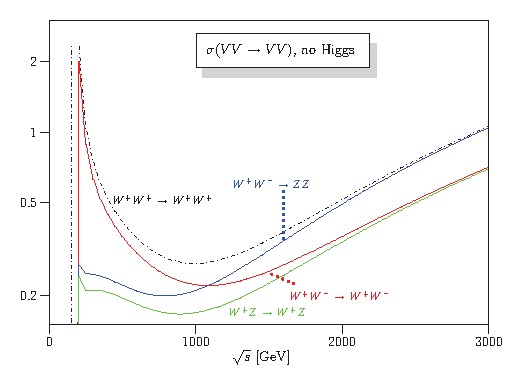
\includegraphics[height=.25\textheight]{figs/ssww_13tev/introduction/vbs_xsec_nohiggs}
  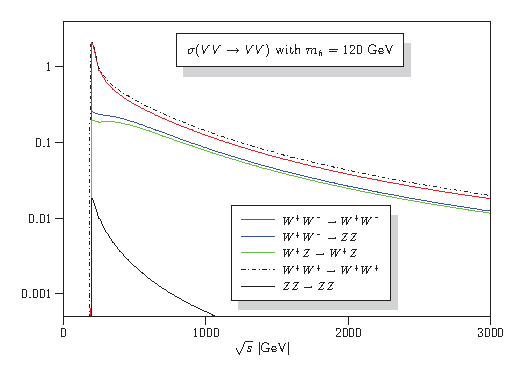
\includegraphics[height=.25\textheight]{figs/ssww_13tev/introduction/vbs_xsec_higgs120}
 
  \caption[Cross sections in nanobarns for five different longitudinally polarized VBS processes as a function of center of mass energy $\sqrt{s}$.  Without a Higgs boson (left), the cross sections grow unbounded with $\sqrt{s}$. With a $120\gev$ Higgs boson (right), the cross sections no longer diverge.]{Cross sections in nanobarns for five different longitudinally polarized VBS processes as a function of center of mass energy $\sqrt{s}$.  Without a Higgs boson (left), the cross sections grow unbounded with $\sqrt{s}$. With a $120\gev$ Higgs boson (right), the cross sections no longer diverge.  Plots taken from~\cite{2008.vbs-resonances-unitarity}.}
  \label{fig:theory_vbs_xsec_higgs}
\end{figure}

